\subsection{Matched-power robustness of the height comparison}
The following paired comparisons vary one uncertain heat path at a time while preserving the 29/11/4 thermocouple layout and solving the actual 88 nonlinear legs and four source ceramic temperature fields at $IV=0.595668$ W, 300 K ambient and 2 mW imposed detector heat. Both geometries receive the same change. The exterior gas path is a lumped proxy, not a resolved native cavity, and may overlap the interstage approximation; its nominal 3 mm effective distance is compared with 1.5 mm. A separate gas case suppresses all three interstage links, while the sink case adds 5 K/W to the original external sink resistance. These are engineering hypotheses, not measured tolerances.

\begin{center}\small\begin{tabular}{lrrr}\toprule
Case & 0.50 mm die (K) & 0.60 mm die (K) & Difference (K) \\ \midrule
V3.20 reference & 219.369 & 215.664 & -3.705 \\
Interstage gas off & 218.898 & 215.159 & -3.739 \\
Outer gas gap 1.5 mm & 219.743 & 216.110 & -3.633 \\
Sink resistance +5 K/W & 221.202 & 217.437 & -3.765 \\
\bottomrule\end{tabular}\end{center}
The taller candidate remains colder at the mount in each displayed paired scenario. The sampled difference ranges from -3.765 to -3.633 K; this is a set of model scenarios, not a statistical interval or a guarantee for a manufactured part. All new cases meet the registered matched-power and independently reconstructed stage and whole-package energy gates. A separate fixed-field copper contact-resistance exercise changes the predicted metal heat paths; it is not an additional coupled temperature prediction. Net88's middle foot is a thermal port, not a series electrical contact. The historical spatial electrical-contact gate remains failed, the gas approximations are not validated native-void solutions, the research P/N specimens are not a matched commercial grade, and continuation above 300 K is assumed.

\begin{figure}[htbp]\centering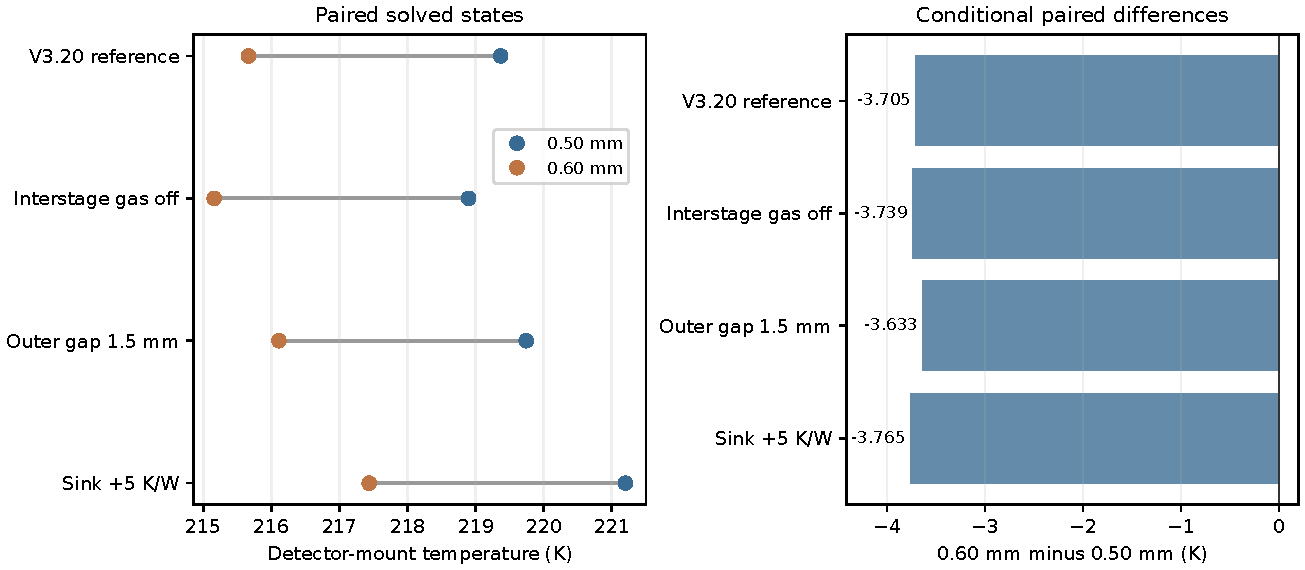
\includegraphics[width=.96\linewidth]{figures/v321_height_robustness.pdf}\caption{Actual matched-power package solutions for the nominal and custom leg heights. Differences are conditional on the specified gas and mounting models, with no interpolation across uncomputed scenarios. The reference pair is the previously archived result; other pairs are new independently audited solutions.}\end{figure}
